\chapter{STRique Repeat Detection}
\label{sec:strique}

Expansions of short tandem repeats are genetic variants that have been implicated in several neuropsychiatric and other disorders, but their assessment remains challenging with current polymerase-based methods. Here we introduce a CRISPR-Cas-based enrichment strategy for nanopore sequencing combined with an algorithm for raw signal analysis. Our method, termed STRique for short tandem repeat identification, quantification and evaluation, integrates conventional sequence mapping of nanopore reads with raw signal alignment for the localization of repeat boundaries and a hidden Markov model-based repeat counting mechanism. We demonstrate the precise quantification of repeat numbers in conjunction with the determination of CpG methylation states in the repeat expansion and in adjacent regions at the single-molecule level without amplification. Our method enables the study of previously inaccessible genomic regions and their epigenetic marks.

\begin{figure}[h]
    \centering
    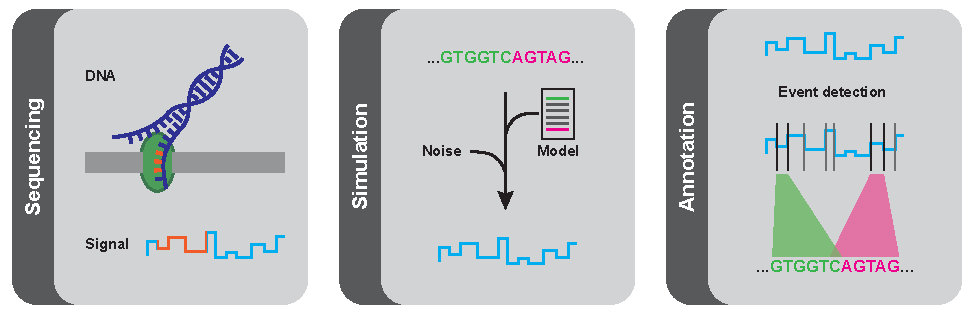
\includegraphics[width=1.0\textwidth]{figures/strique/GA.pdf}
    \label{fig:strique:ga}
\end{figure}



\section{Background}
\label{sec:strique:background}

\section{Data Generation}
\label{sec:strique:data}



\section{Repeat Quantification}
\label{sec:strique:quantification}

\begin{figure}[h]
    \centering
    \includegraphics[width=1.0\textwidth]{figures/strique/Figure1.pdf}
    \captionsetup{format=plain}
    \caption[STRique: generic repeat detection pipeline on raw nanopore signals.]{\textbf{a}, Repeat quantification enabled by raw signal alignment of flanking prefix and suffix regions and HMM-based count on the signal of interest. \textbf{b}, Bioanalyzer electropherogram, decoy alignment, RepeatHMM and STRique counts of synthetic $ (G_{4}C_{2})_{n} $ repeats.}
    \label{fig:strique:1}
\end{figure}

\begin{figure}[h]
    \centering
    \includegraphics[width=1.0\textwidth]{figures/strique/Figure2.pdf}
    \captionsetup{format=plain}
    \caption[STRique: generic repeat detection pipeline on raw nanopore signals.]{\textbf{a}, Repeat quantification enabled by raw signal alignment of flanking prefix and suffix regions and HMM-based count on the signal of interest. \textbf{b}, Bioanalyzer electropherogram, decoy alignment, RepeatHMM and STRique counts of synthetic $ (G_{4}C_{2})_{n} $ repeats.}
    \label{fig:strique:2}
\end{figure}

\section{Base Modification Detection}
\label{sec:strique:modifications}

\begin{figure}[h]
    \centering
    \includegraphics[width=1.0\textwidth]{figures/strique/Figure4.pdf}
    \captionsetup{format=plain}
    \caption[Methylation state analyses at the single-read level.]{\textbf{a}, C9orf72 methylation status in HUES64 as measured by whole-genome bisulfite sequencing. The wild-type (blue) allele and expanded (ex; orange) alleles (with 450 and 750 $ (G_{4}C_{2})_{n} $ repeats (red), respectively) are shown for patient 24/5\#2, as measured by nanopore sequencing. \textbf{b}, Single read nanopore methylation of C9orf72 covering reads from the minus strand (n = 259, 100 and 43 rows per block) sorted by detected repeat length (rows, single read; columns, single CpGs). CpGs with logP ratio $> 2.5$ are considered methylated, while those with logP ratio $< -2.5$ are considered unmethylated. The median methylation difference (95\% CI) and P value (determined by two-sided Wilcoxon rank-sum test on mean promoter CGI methylation) for comparisons were as follows: $ WT-ex450: 3.9 \cdot 10^{-5} (4.8 \cdot 10^{-6} to 3.4 \cdot 10^{-2}), P = 5.3 \cdot 10^{-9}; WT-ex750: 0.56 (0.46-0.64), P < 2.2 \cdot 10^{-16}; ex450-ex750: 0.53 (0.40-0.64), P < 2.2 \cdot 10^{-16}; ***P < 0.001. $ }
    \label{fig:strique:4}
\end{figure}

\section{Summary}
\label{sec:strique:summary}




